%%%%%%%%%%%%%%%%%%%%%%%%%%%%%%%%%%%%%%%%%%%%%%%%%%%%%%%%%%%%%%%%%%
\documentclass[letterpaper, 10pt, conference]{ieeeconf}
\overrideIEEEmargins			% to meet printer requirements
\IEEEoverridecommandlockouts	% to override locked commands

%%%%%%%%%%%%%%%%%%%%%%%%%%%%%%%%%%%%%%%%%%%%%%%%%%%%%%%%%%%%%%%%%%
%REQUIRED PACKAGES%
\usepackage{multirow}
\usepackage{rotating}
\usepackage{float}
\usepackage{caption}
\usepackage{lipsum}
\usepackage{subcaption}
\usepackage{amsmath}
\usepackage{amssymb}
\usepackage{textcomp}
\usepackage{graphicx}
\usepackage{euscript}
\usepackage{ctable}
\graphicspath{{./Figures/}}
\usepackage[nonumberlist,acronym]{glossaries}
\usepackage[hidelinks]{hyperref}

%%%%%%%%%%%%%%%%%%%%%%%%%%%%%%%%%%%%%%%%%%%%%%%%%%%%%%%%%%%%%%%%%%

% correct hyphenation
\hyphenation{temp-orary}

% glossaries
\newacronym{ROS}{ROS}{Robot Operating System}

%%%%%%%%%%%%%%%%%%%%%%%%%%%%%%%%%%%%%%%%%%%%%%%%%%%%%%%%%%%%%%%%%%
\begin{document}

\title{Behavioral Planning Approaches To Improve Autonomous Behaviour During
	Navigation for Mobile Robots Running ROS}

\author{Lukas Evers$^{*,1}$, Umut Uzunoglu$^{1}$, and Ahmed Hussein$^{1}$ \textit{Senior Member, IEEE}%
    \thanks{$^{*}$ Corresponding author }%
    \thanks{$^{1}$ IAV GmbH, Berlin, Germany \newline
		{\tt\small lukas.evers@iav.de, umut.uzunoglu@iav.de, ahmed.hussein@ieee.org}}%
}

\maketitle
\pagestyle{empty}

%%%%%%%%%%%%%%%%%%%%%%%%%%%%%%%%%%%%%%%%%%%%%%%%%%%%%%%%%%%%%%%%%%

\begin{abstract}

This document is a model and instructions for \LaTeX.
This file define the components of your paper [title, text, heads, etc.]. 
*CRITICAL: Do Not Use Symbols, Special Characters, Footnotes, or Math in Paper Title or Abstract.

\end{abstract}

%%%%%%%%%%%%%%%%%%%%%%%%%%%%%%%%%%%%%%%%%%%%%%%%%%%%%%%%%%%%%%%%%%

\section{Introduction}
\label{sec:Introduction}

 Lorem ipsum dolor sit amet, consectetur adipiscing elit. Nam in turpis laoreet magna elementum commodo. Interdum et malesuada fames ac ante ipsum primis in faucibus. Mauris non massa accumsan, molestie velit nec, efficitur leo. Aenean nunc arcu, molestie vitae lectus sit amet, malesuada sagittis lacus. Curabitur fringilla massa ac tellus vestibulum pretium. Sed neque metus, aliquet fringilla tincidunt placerat, vehicula quis justo. Nulla vulputate luctus risus, sed porttitor mauris imperdiet nec. Vestibulum nunc ligula, vestibulum eget nibh sed, volutpat rutrum nisl. Curabitur ultrices nulla urna, et molestie dui rutrum id. Duis faucibus lacinia porttitor. Ut vel commodo nunc~\gls{ROS}~\cite{quigley2009}.

%%%%%%%%%%%%%%%%%%%%%%%%%%%%%%%%%%%%%%%%%%%%%%%%%%%%%%%%%%%%%%%%%%

\section{Related Work}
\label{sec:RelatedWork}

\begin{figure}[ht]
    \centering
    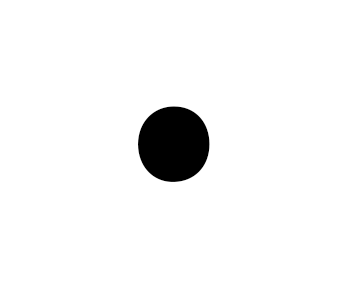
\includegraphics[width=0.9\linewidth]{fig1.png}
    \caption{Figure Caption}
    \label{fig:figureLabel}
\end{figure}

%%%%%%%%%%%%%%%%%%%%%%%%%%%%%%%%%%%%%%%%%%%%%%%%%%%%%%%%%%%%%%%%%%
\section{Proposed Approach}
\label{sec:ProposedApproach}



%%%%%%%%%%%%%%%%%%%%%%%%%%%%%%%%%%%%%%%%%%%%%%%%%%%%%%%%%%%%%%%%%%
\section{Experimental Work}
\label{sec:ExperimentalWork}



%%%%%%%%%%%%%%%%%%%%%%%%%%%%%%%%%%%%%%%%%%%%%%%%%%%%%%%%%%%%%%%%%%

\section{Results and Discussion}
\label{sec:ResultsAndDiscussion}



%%%%%%%%%%%%%%%%%%%%%%%%%%%%%%%%%%%%%%%%%%%%%%%%%%%%%%%%%%%%%%%%%%

\section{Conclusion and Future Recommendations}
\label{sec:Conclusion}


%%%%%%%%%%%%%%%%%%%%%%%%%%%%%%%%%%%%%%%%%%%%%%%%%%%%%%%%%%%%%%%%%%
%\vfill
%\section*{ACKNOWLEDGMENT}

%%%%%%%%%%%%%%%%%%%%%%%%%%%%%%%%%%%%%%%%%%%%%%%%%%%%%%%%%%%%%%%%%%
%\addtolength{\textheight}{-12cm}
%\vspace{10mm}
\bibliographystyle{IEEEtran}
\bibliography{paper}
\end{document}

%%%%%%%%%%%%%%%%%%%%%%%%%%%%%%%%%%%%%%%%%%%%%%%%%%%%%%%%%%%%%%%%%%
